%%% Choose between 16:9 and 4:3 format by commenting out/uncommenting one of the following lines:
\documentclass[aspectratio=169]{beamer} % 16:9
% \documentclass{beamer} % 4:3

%=========================================================================================================================

\usepackage[english]{babel}     % English language
\usepackage[latin1]{inputenc}   % Input encoding
\usepackage{tikz}               % For creating graphics
\usepackage{url}                % For including urls
\usepackage{tabularx}           % For better tables

\usetheme{aig}                  % Set beamer theme

%=========================================================================================================================
\title{Qualit\"at von Wikipedia-Artikeln}

% \author[S. Author]{Some Author}
\institute{Artificial Intelligence Group,\\
University of Hagen, Germany}
\date{\today}
%=========================================================================================================================
\logo{
\includegraphics[width=3cm]{figures/logoaig.png}}
%=========================================================================================================================

\begin{document}

%=========================================================================================================================

% frame
% block
% alertblock
% exampleblock

% \highlight{}
% \darkhighlight{}
% \yellowhighlight{}
% \mathhighlight{}
% \darkmathhighlight{}
% \yellowmathhighlight{}

% appendix

\begin{frame}
    \titlepage
\end{frame}
\nologo

\section{Problemstellung}

\begin{frame}{Problemstellung}
    \begin{block}{Problemstellung}
        Das Ziel dieses Projekts ist die Entwicklung von Modellen zur automatisierten Klassifikation von Wikipedia-Artikeln als promotional (werblich) oder nicht-promotional. Wikipedia strebt nach objektiven und neutralen Inhalten; daher ist die Identifizierung von Artikeln mit werbenden Charakter von gro\ss{}er Bedeutung, um die sachliche Qualit\"at der Plattform zu gew\"ahrleisten.
    \end{block}
\end{frame}

\section{Daten}

\begin{frame}{Daten}
    \begin{itemize}
        \item 54116 gelabelte Wikipedia Artikel

        \item 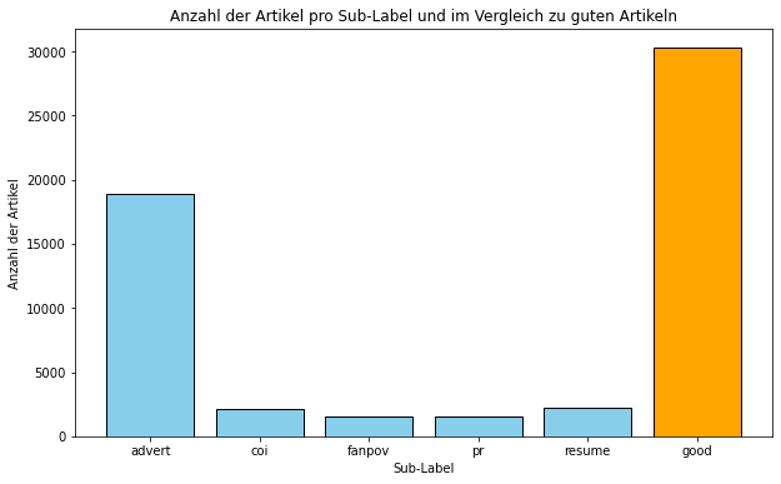
\includegraphics[width=10cm]{figures/distribution_multiple_classes.png}
    \end{itemize}
\end{frame}

\section{Ans\"atze}

\subsection{Logistische Regression}

\begin{frame}{Logistische Regressionn}

\end{frame}

\subsection{Support Vector Machine}

\begin{frame}{Support Vector Machine}

\end{frame}

\subsection{Bayes Klassifikator}

\begin{frame}{Bayes Klassifikator (1)}
    \begin{block}{Datenvorverarbeitung}
        \begin{itemize}
            \item Entfernen von Nicht-Wort-Zeichen
            \item Umwandlung in Kleinbuchstaben
            \item Entfernung von f\"uhrenden und folgenden Leerzeichen
            \item Beibehaltung von Stoppw\"ortern und Zahlen (KPIs nicht beeinflusst)
        \end{itemize}
    \end{block}
\end{frame}
\begin{frame}{Bayes Klassifikator (2)}
    \begin{block}{Methode}
        \begin{itemize}
            \item Textrepr\"asentation mittels TF-IDF-Vektorisierung:
                  \begin{itemize}
                      \item Maximale Anzahl von Features: 10.000
                      \item n-Gramm-Bereich: Unigramme (1,1)
                      \item Minimale Dokumentenfrequenz (\texttt{min\_df}): 0.001
                      \item Maximale Dokumentenfrequenz (\texttt{max\_df}): 0.9
                  \end{itemize}
            \item Einstellung des Gl\"attungsparameters \(\alpha = 1.0\)
            \item \textbf{Bin\"are Klassifikation}:
                  \begin{itemize}
                      \item Einsatz von \texttt{MultinomialNB} f\"ur die Klassifikation zwischen promotional und nicht-promotional Artikeln
                  \end{itemize}
            \item \textbf{Multilabel-Klassifikation}:
                  \begin{itemize}
                      \item Verwendung von \texttt{OneVsRestClassifier} mit \texttt{MultinomialNB} f\"ur die Klassifikation in mehrere Klassen
                      \item Behandlung des Klassenungleichgewichts durch Oversampling mit \texttt{RandomOverSampler}
                  \end{itemize}
        \end{itemize}
    \end{block}
\end{frame}
\begin{frame}{Bayes Klassifikator (3)}
    \begin{block}{Ergebnisse}
        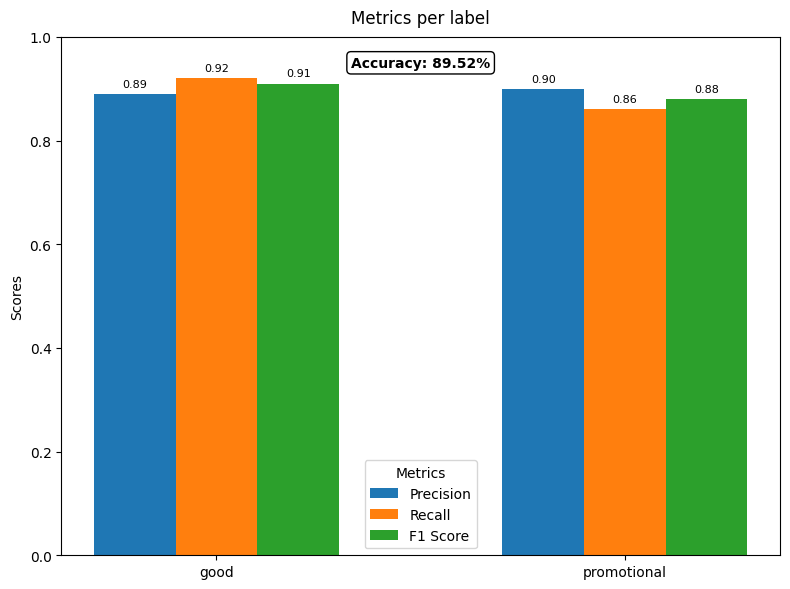
\includegraphics[width=6.8cm]{figures/evaluation_nbb.png} 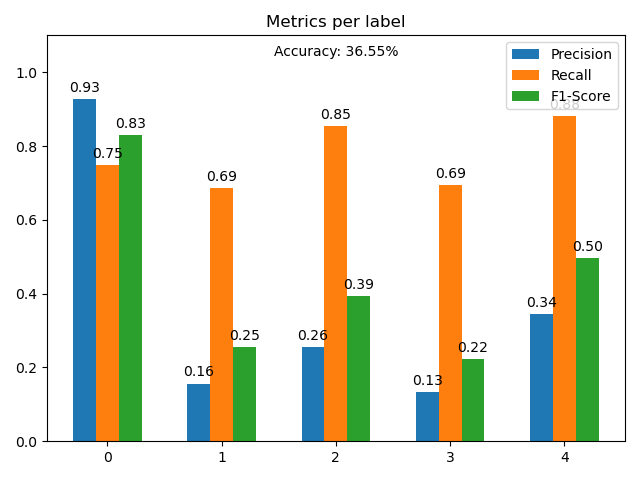
\includegraphics[width=6.8cm]{figures/evaluation_nbm.png}
    \end{block}
\end{frame}

\subsection{Convolutional Neural Network}

\begin{frame}{Convolutional Neural Network}

\end{frame}
\end{document}
